% Created 2025-01-05 Sun 18:06
% Intended LaTeX compiler: lualatex
\documentclass[11pt]{article}
\usepackage{fontspec}
\usepackage{graphicx}
\usepackage{lilyglyphs}
\usepackage{graphicx}
\usepackage{longtable}
\usepackage{wrapfig}
\usepackage{rotating}
\usepackage[normalem]{ulem}
\usepackage{amsmath}
\usepackage{amssymb}
\usepackage{capt-of}
\usepackage{hyperref}
\usepackage[cm]{fullpage}
\usepackage[headheight=15pt, headsep=10pt, top=1in, bottom=1in, left=0.75in, right=0.75in]{geometry} % Ensure sufficient header space
\usepackage{fancyhdr}
\pagestyle{fancy}
\fancyhf{}
\fancyhead[L]{\textbf{\title}} % Use the Org #+TITLE
\fancyhead[R]{\textbf{\author}} % Use the Org #+AUTHOR
\fancyfoot[C]{\thepage}
\renewcommand{\headrulewidth}{0.4pt} % Optional: Add a horizontal rule below the header
\makeatletter
\let\ps@plain\ps@fancy % Apply "fancy" style to the first page
\let\maketitle\relax % Suppress default title/author rendering
\makeatother
\author{Bartev}
\date{\today}
\title{ii-V Snippets}
\hypersetup{
 pdfauthor={Bartev},
 pdftitle={ii-V Snippets},
 pdfkeywords={},
 pdfsubject={},
 pdfcreator={Emacs 29.4 (Org mode 9.6.15)}, 
 pdflang={English}}
\begin{document}

\maketitle

\section*{Basic ii-V-I phrases}
\label{sec:org40932d7}
\subsection*{In E-flat}
\label{sec:org2b88fd7}
\begin{center}
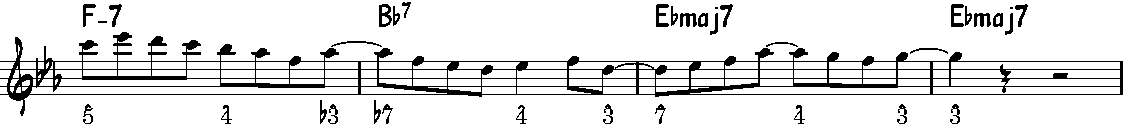
\includegraphics[width=.9\linewidth]{e-flat.pdf}
\end{center}

\subsection*{G maj}
\label{sec:org2d51a65}
\begin{center}
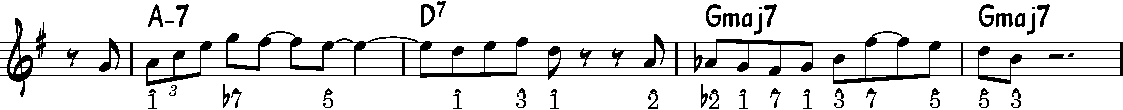
\includegraphics[width=.9\linewidth]{g_maj.pdf}
\end{center}

\subsection*{G maj (variation 2)}
\label{sec:org1eb16de}
\begin{center}
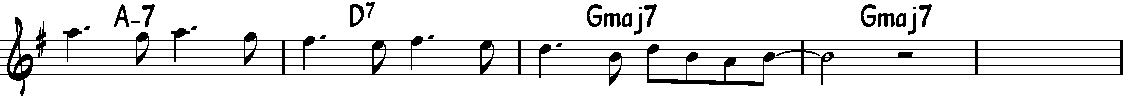
\includegraphics[width=.9\linewidth]{g_maj_v2.pdf}
\end{center}
\end{document}
